\documentclass{oci}
\usepackage[utf8]{inputenc}
\usepackage{lipsum}
\usepackage{subcaption}

\title{La leyenda de Zolda}
\codename{zolda}

\begin{document}
\begin{problemDescription}
  \emph{La leyenda de Zolda} es una popular saga de videojuegos con ya más de 19
  títulos, incluyendo aclamadas entregas como \emph{La zampoña del tiempo},
  \emph{La princesa del amanecer}, \emph{Un enlace al futuro} y \emph{Aliento de
  la civilización}.

  En la última versión del videojuego existe una modalidad donde el personaje
  principal, Lonk, debe enfrentarse a una horda de \emph{meblins}.
  En esta modalidad el escenario corresponde a un plano cartesiano como el que
  se muestra en la figura de más abajo.
  Nuestro héroe se encontrará siempre en la coordenada $(0,0)$ y los meblins
  pueden estar en cualquier coordenada distinta a esta.
  En la figura de más abajo Lonk está representado con una estrella y los meblins
  mediante puntos.
  \vspace{-0.5em}
  \begin{center}
  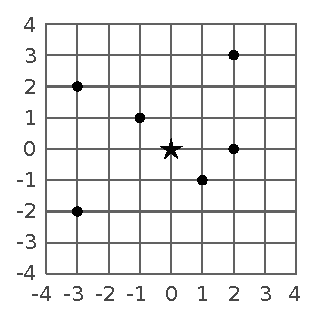
\includegraphics[scale=0.9]{zolda}
  \end{center}
  \vspace{-0.5em}
  Para pasar de nivel Lonk debe eliminar al menos $K$ meblins del escenario
  usando su poderoso \emph{ataque de giro}.
  Con este ataque Lonk puede de un solo golpe dañar todo a su alrededor.
  Dependiendo la potencia que use, Lonk puede variar el radio de alcance de su
  ataque.
  Específicamente, si Lonk escoge un radio $R$ eliminará a todos los meblins que
  se encuentren dentro de este radio.
  Con el fin de reservar energía para el futuro una buena estrategia es siempre
  utilizar el menor radio con el cuál es posible eliminar a los $K$ meblins.
  Por ejemplo, en el escenario mostrado anteriormente, si el objetivo es eliminar
  $K=3$ meblins, el menor radio con que esto es posible es 2.

  \begin{figure}[h]
    \centering
    \begin{subfigure}{0.3\textwidth}
      \centering
      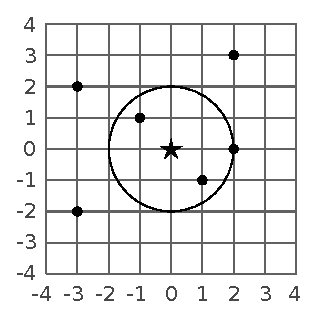
\includegraphics[scale=0.8]{zolda2}
      \caption*{Con R=2 Zolda elimina los 3 meblins requeridos.}
    \end{subfigure}
    \hspace{3em}
    \begin{subfigure}{0.3\textwidth}
      \centering
      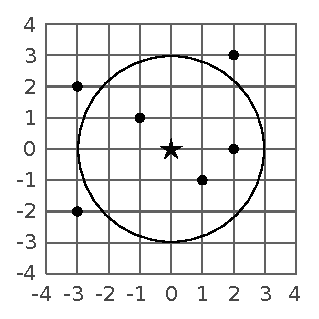
\includegraphics[scale=0.8]{zolda3}
      \caption*{Con R=3 Zolda elimina también 3 meblins.}
    \end{subfigure}
  \end{figure}

\end{problemDescription}

\begin{inputDescription}
  La entrada está descrita en varias líneas.
  La primera linea contiene dos enteros $N$ y $K$ ($0<K\leq N$) correspondientes a la cantidad
  de meblins en el escenario y la cantidad que hay que eliminar para pasar de nivel.
  A continuación se entregan $N$ lineas cada una conteniendo dos enteros $X_i$ y
  $Y_i$ que representan las coordenadas del i-ésimo meblin.
  Se garantiza que no habrá dos meblins en la misma posición y que ningún
  meblin estará en la misma posición que Zolda.
\end{inputDescription}

\begin{outputDescription}
  La salida debe corresponder a un único entero correspondiente al radio $R$
  mínimo con el cual es posible eliminar $K$ meblins.
\end{outputDescription}

\begin{scoreDescription}
\score{12} Se probarán varios casos donde $0 < N \leq 100$ y $-10^3 \leq X_i,Y_i  \leq 10^3$.
\score{27} Se probarán varios casos donde $100 < N \leq 10^5$ y $-10^4 \leq X_i, Y_i \leq 10^4$.
\score{28} Se prabarán varios casos donde $100 < N \leq 10^5$, $-10^9 \leq X_i \leq 10^9$ y $Y_i = 0$.
\score{33} Se probarán varios casos donde $100 < N \leq 10^5$ y $-10^9 \leq X_i, Y_i \leq 10^9$.
\end{scoreDescription}

\begin{sampleDescription}
\sampleIO{sample-1}
\sampleIO{sample-2}
\sampleIO{sample-3}
\end{sampleDescription}

\end{document}
